%%%%%%%%%%%%%%%%%%%%%%%%%%%%%%%%%%%%%%%%%
% Short Sectioned Assignment LaTeX Template Version 1.0 (5/5/12)
% This template has been downloaded from: http://www.LaTeXTemplates.com
% Original author:  Frits Wenneker (http://www.howtotex.com)
% License: CC BY-NC-SA 3.0 (http://creativecommons.org/licenses/by-nc-sa/3.0/)
%%%%%%%%%%%%%%%%%%%%%%%%%%%%%%%%%%%%%%%%%

%----------------------------------------------------------------------------------------
%	PACKAGES AND OTHER DOCUMENT CONFIGURATIONS
%----------------------------------------------------------------------------------------

\documentclass[paper=a4, fontsize=11pt]{scrartcl} % A4 paper and 11pt font size

% ---- Entrada y salida de texto -----


\usepackage[dvipsnames]{xcolor}
\usepackage{colortbl}
\usepackage{verbatim}
\usepackage{booktabs}
\usepackage{enumitem}
\newlist{subquestion}{enumerate}{1}
\setlist[subquestion,1]{label=(\alph*)}
\usepackage[T1]{fontenc} % Use 8-bit encoding that has 256 glyphs
\usepackage[utf8]{inputenc}
%\usepackage{fourier} % Use the Adobe Utopia font for the document - comment this line to return to the LaTeX default

% ---- Idioma --------

\usepackage[spanish, es-tabla]{babel} % Selecciona el español para palabras introducidas automáticamente, p.ej. "septiembre" en la fecha y especifica que se use la palabra Tabla en vez de Cuadro

% ---- Otros paquetes ----

\usepackage{url} % ,href} %para incluir URLs e hipervínculos dentro del texto (aunque hay que instalar href)
\usepackage{amsmath,amsfonts,amsthm} % Math packages
%\usepackage{graphics,graphicx, floatrow} %para incluir imágenes y notas en las imágenes
\usepackage{graphics,graphicx, float, subfig} %para incluir imágenes y colocarlas

% Para hacer tablas comlejas
%\usepackage{multirow}
%\usepackage{threeparttable}

%\usepackage{sectsty} % Allows customizing section commands
%\allsectionsfont{\centering \normalfont\scshape} % Make all sections centered, the default font and small caps

\usepackage{fancyhdr} % Custom headers and footers
\pagestyle{fancyplain} % Makes all pages in the document conform to the custom headers and footers
\usepackage{eurosym} % Para poder añadir el símbolo del euro
\fancyhead{} % No page header - if you want one, create it in the same way as the footers below
\fancyfoot[L]{} % Empty left footer
\fancyfoot[C]{} % Empty center footer
\fancyfoot[R]{\thepage} % Page numbering for right footer
\renewcommand{\headrulewidth}{0pt} % Remove header underlines
\renewcommand{\footrulewidth}{0pt} % Remove footer underlines
\setlength{\headheight}{13.6pt} % Customize the height of the header

\numberwithin{equation}{section} % Number equations within sections (i.e. 1.1, 1.2, 2.1, 2.2 instead of 1, 2, 3, 4)
\numberwithin{figure}{section} % Number figures within sections (i.e. 1.1, 1.2, 2.1, 2.2 instead of 1, 2, 3, 4)
\numberwithin{table}{section} % Number tables within sections (i.e. 1.1, 1.2, 2.1, 2.2 instead of 1, 2, 3, 4)

\setlength\parindent{0pt} % Removes all indentation from paragraphs - comment this line for an assignment with lots of text

\newcommand{\horrule}[1]{\rule{\linewidth}{#1}} % Create horizontal rule command with 1 argument of height


\usepackage{algpseudocode}
\usepackage[spanish]{babel}
\usepackage{varwidth}
\usepackage{hyperref}

\selectlanguage{spanish} 
\usepackage[spanish,onelanguage]{algorithm2e} %for psuedo code
\usepackage[lmargin=3.81cm,tmargin=2.54cm,rmargin=2.54cm,bmargin=2.52cm]{geometry}
%\usepackage{listings}
%\usepackage{dsfont}

%----------------------------------------------------------------------------------------
%	TÍTULO Y DATOS DEL ALUMNO
%----------------------------------------------------------------------------------------

\title{	
\normalfont \normalsize 
\textsc{\textbf{Metaheurísticas(2019-2020)} \\ Doble Grado en Ingeniería Informática y Matemáticas \\ Universidad de Granada} \\ [25pt] % Your university, school and/or department name(s)
\horrule{0.5pt} \\[0.4cm] % Thin top horizontal rule
\huge Técnicas de Búsqueda Local y Algoritmos Greedy \\ para el Problema de la Máxima Diversidad  (MDP) \\ % The assignment title
\horrule{2pt} \\[0.5cm] % Thick bottom horizontal rule
}
\author{Alberto Jesús Durán López \\ 
DNI: 54142189-M \\
albduranlopez@gmail.com \\
\hfill \break \hspace{1cm}\\
Grupo Jueves, 17:30 - 19:30 } % Nombre y apellidos


\date{\normalsize\today} % Incluye la fecha actual

%----------------------------------------------------------------------------------------
% DOCUMENTO
%----------------------------------------------------------------------------------------

\begin{document}

\maketitle % Muestra el Título

\newpage %inserta un salto de página

\tableofcontents % para generar el índice de contenidos

% \listoffigures

% \listoftables

\newpage


\section{Introducción}
\hspace{1.5cm} Durante el transcurso de la asignatura trabajaremos con el problema de la máxima diversidad \textit{(Max Diversity Problem)}. 


En particular, en esta práctica estudiaremos el funcionamiento de \textit{Técnicas de Búsqueda Local y de los Algoritmos Greedy} para la resolución del problema en cuestión. \\
Comentaremos todos los pasos y problemas encontrados, detallando minuciosamente todos los detalles y solución a los mismos. \\

Además, se incorporarán tablas para mostrar los resultados de ambas ejecuciones y  gráficas para contrastar ambos modelos (optimización, costes y desviación).


\section{Problema de la máxima Diversidad}
\hspace{1.5cm} El problema de la máxima diversidad (\textit{maximum diversity problem}, MDP) es un problema de optimización combinatoria consistente en seleccionar un subconjunto de m elementos ($|M|=m$) de un conjunto inicial N de n elementos (con $n>m$) de forma que se maximice la diversidad entre los elementos escogidos. \\


El \textbf{MDP} se puede formular como: \\


\[
\text{Maximizar:   }  z_{MS}(x) = \sum_{i=1}^{n-1} \sum_{j=i+1}^{n} d_{ij}x_i x_j
\]



\[
\text{Sujeto a: } \sum_{i=1}^{n} x_i=m \hspace{0.2cm} \text{ con } x_i=\{0,1\} \text{, } i=1,...,n  \hspace{0.5cm} \text{donde: }
\]


\begin{itemize}
	\item x es una solución al problema que consiste en un vector binario que indica los m elementos seleccionados.
	\item $d_{ij}$ es la distancia existente entre los elementos $i$ y $j$
	
\end{itemize}


\begin{figure}[H]
	\centering
	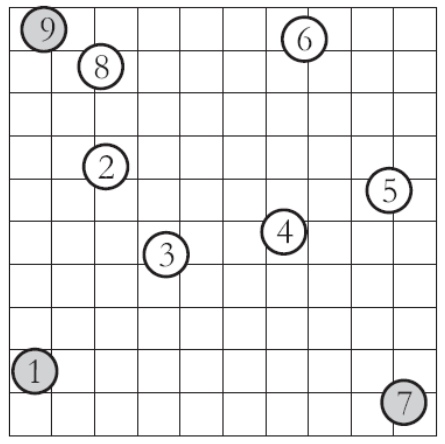
\includegraphics[scale=0.35]{img/mdp.png}
	\caption{MDP-Maximum Diversity Problem}
\end{figure}


\section{Datos y casos considerados}
\hspace{1.5cm} Las ejecuciones se han realizado en un ordenador \texttt{Intel(R) Core(TM) i7-1065G7 CPU @ 1.30GHz, 16GB RAM, 512 SSD}. \\

Para la realización de las prácticas usaremos el lenguaje de programación \texttt{C++} ya que se deben probar muchos ejemplos y la ejecución es más rápida al ser un lenguaje de programación compilado. \\

Se utilizarán \textbf{30 casos} seleccionados de varios de los conjuntos de instancias disponible en la \href{http://www.optsicom.es/mdp/}{MDPLIB}, 10 pertenecientes al grupo \texttt{GKD} con distancias Euclideas, n=500 y m=50 \textit{(GKD-c\_11\_n500\_m50 a GKD-
c\_20\_n500\_m50)}, 10 del grupo \texttt{MDG} con distancias reales en [0,1000], n=500 y m=50
\textit{(MDG-b\_1\_n500\_m50 a MDG-b\_10\_n500\_m50)}; y otras 10 del grupo \texttt{MDG} con distancias enteras en {0,10}, n=2000 y m=200 \textit{(MDG-a\_31\_n2000\_m200 a MDG-
a\_40\_n2000\_m200)}. \\

Tras la ejecución de los algoritmos se han rellenado dos tablas con sus respectivos resultados \textit{(MDP\_greedy.ods, MDP\_BL.ods)} y, además, un archivo extra donde se ha añadido un resumen acompañado con gráficas que explicaremos a lo largo de la práctica. \textit{(gráficas.ods)}. Adicionalmente, se han añadido a la entrega dos ficheros: \textit{Output.txt} y \textit{Output\_O2.txt} donde se han volcado los resultados de la ejecución de todos los ficheros requeridos con y sin optimización \texttt{-O2}, respectivamente.



\section{Algoritmo}

 \hspace{1.5cm }En la siguiente sección, estudiaremos los algoritmos implementados, \textit{Greedy} y \textit{Búsqueda Local}.


\subsection{Descripción de la Función Objetivo}

Tanto el algoritmo \textit{Greedy} como \textit{Búsqueda Local} hacen uso de la misma función objetivo, la comentada en el punto (2) anterior y cuyo pseudocódigo mostramos a continuación:


\begin{figure}[H]
	\centering
	\begin{minipage}{.9\linewidth}
		
		
		
		\begin{algorithm}[H] 
			
			\caption{Evaluar solución}
			\SetAlgoLined
			
			\KwData{\textbf{CosteEstimado}(\textit{vector sel, matriz distancias)}}
			
			\Begin{
				
				\textit{suma $\leftarrow$ 0} \;
				
				
				\For{i in $|sel|-1$}{
					\For{$j \leftarrow$ $i+1$ in $|sel|$}{
						$ suma \leftarrow distancias[i][j] + suma$ \;
					}
					
				}
				
				\Return $suma$
			}
			
		\end{algorithm} 
		
	\end{minipage}
\end{figure}


\newpage
Sin embargo, en el algoritmo \textit{Búsqueda Local} realizamos una pequeña modificación ya que es necesario calcular la contribución de cada elemento independientemente, y por tanto, el coste de la solución se podría llamando a la anterior función \texttt{CosteEstimado} o bien sumando las contribuciones independientes de todos los elementos que forman la solución.

\begin{figure}[H]
	\centering
	\begin{minipage}{.9\linewidth}
		
		
		
		\begin{algorithm}[H] 
			
			\caption{Contribución Independiente}
			\SetAlgoLined
			
			\KwData{\textbf{ContribucionIndep}(\textit{int ind, vector sel, matriz distancias)}}
			
			\Begin{
				\textit{suma $\leftarrow$ 0} \;
				
				\For{j in sel}{
					$ suma \leftarrow distancias[ind][j] + suma$ \;	
				}
				
				\Return $suma$
			}
			
		\end{algorithm} 
		
	\end{minipage}
\end{figure}









\subsection{Greedy}
\hspace{1.5cm} El algoritmo \textit{greedy} del MDP se basa en la heurística de ir seleccionando los elementos más lejanos a los previamente seleccionados. Para ello, se parte del elemento más alejado del resto en el conjunto de elementos. En los $m-1$ pasos siguientes se va escogiendo el elemento más lejano a los elementos seleccionados hasta el momento. Cabe destacar que en nuestros casos del problema no disponemos de los valores concretos de los elementos sino solo de las distancias entre ellos, luego el algoritmo está levemente modificado respecto al original.  \\

Añadimos primeramente el código que devuelve la distancia entre los dos conjuntos que utiliza esta heurística (\texttt{Dist2Conj}), es decir, el conjunto de \textit{Seleccionados}, de tamaño m y el conjunto de \textit{No Seleccionados}, de tamaño $n-m$.
A partir del vector de seleccionados y no seleccionados, recorremos ambos contenedores para obtener así el valor mínimo de la distancia de cada $s_i$ a $s_j$ con $s_i \in Unsel$ y  $s_j \in Sel$. Una vez llenado el vector con estos valores, devolvemos el máximo de todos ellos. \\




\begin{figure}[H]
	\centering
	\begin{minipage}{.9\linewidth}
		
		

\begin{algorithm}[H] 

	\caption{Dist2conj (Distancia entre los dos conjuntos, Sel-UnSel)}
	\SetAlgoLined
	
	\KwData{\textbf{Dist2Conj}(\textit{vector Sel, vector unSel, matriz Distancias)}}
	
	\Begin{
		
		\textit{double suma $\leftarrow$ 0} \;
	
		
		\For{it in unSel}{
			\For{it2 in Sel}{
				$ suma \leftarrow distancias[*it][*it2] + suma$ \;
			}
			
		
			\If{suma>maximo}{
				
				$maximo  \leftarrow suma $\;
				$indice  \leftarrow *it $\;				
			}
				
			$suma  \leftarrow 0 $ \;
		}
	
		\Return $indice$
	}
	
	
\end{algorithm} 




\end{minipage}
\end{figure}

\hfill


Ahora bien, nos centramos en la función principal de nuestro algoritmo, la llamaremos \textit{Greedy}. 
Dividiremos su implementación en dos partes:

\begin{enumerate}
	\item Insertamos en el vector \textbf{acum} la distancia acumulada de cada elemento de la matriz de distancias al resto.
	
	Claramente, la matriz de distancias
	resultante tras leer los ficheros \texttt{.txt} proporcionados es simétrica y por ende, sólo es necesario rellenar la diagonal superior o inferior. Sin embargo, para facilitar las operaciones, la rellenamos entera y, la distancia acumulada se puede calcular con un doble bucle \texttt{for}.
	
	
	
	
	\item Introducimos en el vector de 
	seleccionados aquellos elementos que devuelvan la distancia entre el vector de \textit{seleccionados} y \textit{no seleccionados}. Estos índices se obtienen llamando a la función \texttt{Dist2Conj}, previamente explicada. \\
	

\begin{figure}[H]
	\centering
	\begin{minipage}{.7\linewidth}
		
		
	\begin{algorithm}[H] 
		\caption{Greedy MDP}
		\SetAlgoLined
		
		\KwData{\textbf{Greedy}(\textit{integer m, matriz distancias})}
		
		\Begin{
			$vector$ $sel, unSel$ \;
			
			$vector$ $acum \leftarrow$ \texttt{DistanciaAcumulada}$(distancias)$
			
			$integer$   $s_i \leftarrow \texttt{max}(acum)$ \;
			
			$sel \leftarrow$ $sel \cup s_i$ \;
			$unSel \leftarrow unSel - \{s_i\}$ \;
			
			\While{$|sel| < m $}{
				$s_i^* \leftarrow \texttt{dist2conj}(sel, unSel, distancias)$\;
				
				$sel \leftarrow sel \cup s_i^*$ \;
				
				$unsel \leftarrow unsel-{s_i^*}$\;
				
			}
		}
		
		
	\end{algorithm}

\end{minipage}
\end{figure}

	
\end{enumerate}





\newpage

\subsection{Búsqueda Local}
Para la implementación del algoritmo de Búsqueda Local, consideramos el esquema disponible en el \textit{Seminario 2} de la asignatura. Explicaremos el algoritmo con minuciosidad adjuntando trozos de psudocódigo reflejando lo realizado. La semilla usada para todas las ejecuciones ha sido \texttt{54142189}, pudiéndose ésta indicar en la ejecución del archivo en cuestión.

\begin{enumerate}
	\item 
	Primeramente partimos de una solución obtenida de forma aleatoria, es decir, con un vector \textit{sel} de tamaño $m\leq n$ donde n representa el orden de la matriz de distancias. 
	
	
	
	
	
	
	\begin{figure}[H]
		\centering
		\begin{minipage}{.7\linewidth}
			
			
	
	\begin{algorithm}[H] 
		\caption{SolucionInicial}
		\SetAlgoLined
		
		\KwData{$\textbf{SolucionInicial}(integer$ $n, integer$ $m)$}
		
		\Begin{
			
			
			$unordered\_set$ $sel$ \;
			
			
			\While{$|sel|<m$}{
				$random = rand()\%n$ \;
				$sel \leftarrow s_{random}$ \;
			}
			
			\textbf{devolver} sel \;
		}
	
	\end{algorithm}
	
	
			
			
			
		\end{minipage}
	\end{figure}
	
	La estructura usada para almacenar los índices de los elementos en seleccionados es \textit{unordered\_set} que, como bien sabemos, no almacena repetidos y, como consecuencia, la solución inicial estará formada por m índices diferentes.
		
	
	\item 
	\texttt{Función de Generación j}: En cada iteración, seleccionamos el elemento del vector de seleccionados \texttt{i} que menor  contribución aporte y lo intercambiamos por otro elemento \texttt{j} del entorno con mejor heurística.
	
	En el contenedor \textit{todasJ} introducimos todos los índices \texttt{j} que se han generado, de forma que si la nueva solución no mejora respecto a la anterior, no se vuelve a generar el mismo valor \texttt{j} y, como consecuencia, no se generan valores repetidos. 
	
	


\begin{figure}[H]
	\centering
	\begin{minipage}{.7\linewidth}
		
	\begin{algorithm}[H] 


		\caption{Generar índice j}
		\SetAlgoLined
		
		\Begin{
			$integer$ $j$ \;
			
			
			\While{$j\in sel $ \hspace{0.06cm} or \hspace{0.06cm} se ha generado antes}{
				$j \leftarrow$ \textit{generar nuevo j} \;
			}
			$todasJ \leftarrow todasJ \cup j $ \;
		
		
			
			\Return{j} \;
		}

		

	\end{algorithm}
		
	\end{minipage}
\end{figure}
	
	
	\newpage
	\textbf{Descripción del entorno:} 
	En nuestro problema MDP, el parámetro \texttt{i} indica el índice del elemento que se eliminará de la solución y el j por cual se sustituirá. Por tanto, las opciones para \texttt{i} serán \texttt{m} (los m elementos seleccionados) y las opciones para \texttt{j} serán \texttt{n-m} (los elementos disponibles en \textit{no seleccionados}), por tanto, el entorno estará formado por \texttt{m$\cdot$(n-m)} elementos.
	
	Si el intercambio es favorable, es decir, si el coste de la nueva solución (sumando las distancias del nuevo elemento y restando las del elemento anterior) es mayor que la anterior, aceptamos el intercambio. En caso contrario, rechazamos.
	
	Repetiremos este proceso hasta que se realicen 100.000 evaluaciones de la función objetivo o cuando no encuentre mejora en el entorno.
	
	
	Retomando la explicación del contenedor \textit{todasJ}, explicaremos su utilidad en la función para evaluar el entorno.
	Si este contenedor está vacío significa que el anterior intercambio(i,j) fue favorable y sólo es necesario encontrar el \textit{$s_i$} que menor contribución aporte.
	En caso contrario, si \textit{todasJ} está lleno (tiene n-m elementos) hay que pasar al \textbf{siguiente} elemento que menor contribución aporte.
	
	
	\begin{figure}[H]
		\centering
		\begin{minipage}{.75\linewidth}
			
	\begin{algorithm}[H] 
		\caption{EvaluaVecinos }
		\SetAlgoLined
		
		\KwData{\textbf{EvaluaVecinos}\textit{(pair<vector,int> inicial, $\text{  } \hspace{3cm}$matriz distancias)}}
		
		
		\Begin{
			
			\textit{ mejora $\leftarrow$ True}\;
			\textit{ eval $\leftarrow$0, siguienteMin $\leftarrow$ 0} \;
			
			\break \hfill
			
			
			\While{\textit{eval<100.000 and mejora}}{
				
				\If{$|todasJ|=0$}{
					$s_i$ $\leftarrow$ \texttt{min\_element(contribuciones)} \;
					\textit{siguienteMin $\leftarrow$ 0} \;					
				}
				\textbf{else} \If{$|todasJ| \not=0$ and  $siguienteMin<m$}{
					\textit{siguienteMin $\leftarrow$ siguienteMin+1} \;
					
					$s_i$ $\leftarrow$ \texttt{next\_min\_element(contribuciones)} \;
					
				}
	
				
				\textbf{else} \If{entorno explorado}{
					$mejora$ $\leftarrow$ \textit{False} \;
					\textbf{return} \;
				}
				
				
				
				\break \hfill
				
				$salir \leftarrow$ False, $c \leftarrow 0$ \;
				
				\While{$c< n-m$ and not salir}{
				
					\textit{Genera elemento válido j} \;
					
					\If{\texttt{Contrib($s_j$)}>\texttt{Contrib($s_i$)}}{

						\textit{Int(sel, i, j)} \;
						$salir \leftarrow$ True\;
						$coste\leftarrow coste + contribNueva - contribAntigua$ 
					}
					$c\leftarrow c+1$\;
					$eval\leftarrow eval+1$\;
			
				}
				
			
			
			
			
			
			}
		}
		
		
	\end{algorithm}
		\end{minipage}
	\end{figure}


	\newpage
	Resumidamente, el algoritmo a seguir es el siguiente: 
	\begin{itemize}
		\item Antes de llamar a la función \texttt{EvaluaVecinos}, tenemos una solución aleatoria. En cada iteración tomamos el elemento \texttt{$s_i$} que menor contribución aporte de todos y el objetivo será generar el elemento  \texttt{$s_j$} a intercambiar. 
		
		\item Primero, la búsqueda del indice \texttt{j} se hará tras fijar \texttt{$i$}.
		Haciendo uso de la función \texttt{rand()}, generaremos valores  que no se hayan generado para el valor \texttt{$i$} fijado. Si la contribución del nuevo elemento es mayor que la del anterior, aceptamos el cambio.
		El conjunto de \texttt{$j$} generados se guardaran en el vector \texttt{$todasJ$} de forma que no se generen dos índices iguales y así se pueda generar todo el entorno de forma correcta y sin repetidos.
		
		\item Si para el valor \texttt{$i$} que menos contribución aporte no se encuentra ningún \texttt{$j$} cuyo intercambio sea aceptado, pasaremos al siguiente \texttt{$i$} que menor contribución aporte. Este proceso, que se indica en el algoritmo anterior en el segundo if, cuando $|todasJ| \not=0$ y \textit{siguienteMin<m}, es decir, para cuando el valor \texttt{$i$} no se encuentre ningún \texttt{$j$} a intercambiar y cuando no se hayan recorrido los m índices de \textit{seleccionados}, respectivamente.
		Así pues, este proceso se repetirá hasta recorrer todos los valores posibles de \texttt{$n$} y \texttt{$m$}, es decir, $m \cdot (n-m)$
		
		\item Por último, cuando se haya recorrido todo el vector de \textit{seleccionados} y no haya encontrado mejora en el entorno, saldremos de la función.
	\end{itemize} 



	
	\subsubsection{Optimización}
	
	Adelantamos que únicamente el algoritmo de \textit{Búsqueda Local} con los ficheros \texttt{MDG-a} tiene un tiempo de ejecución algo superior, en torno a un segundo más que el resto. Esto es debido a que en dichos ficheros se trabaja con una matriz de distancias regular de tamaño 2000 y, por ello, el entorno es mayor.
	
	
	Para reducir el tiempo de ejecución, se ha compilado el código con la opción de optimización -O2 y, además, se ha realizado una factorización del coste para obtener una mayor eficiencia.
	
	En cada iteración, podemos calcular la diferencia de costes entre las dos soluciones recalculando todas las distancias de la función objetivo, sin embargo, esto no es necesario ya que como únicamente añadimos y quitamos 1 elemento, basta con sumar y restar la distancia del nuevo y del viejo elemento al resto de elementos seleccionados, respectivamente. Además, combinamos la factorización del coste con el cálculo de la contribución de los elementos para mejorar más aún la eficiencia.
	
	
	
	
	
	
	
	\newpage
	
	Mostramos, por último, la función llamada \texttt{BusquedaLocal}. En ella, vemos que la estructura elegida para almacenar la solución ha sido un \textit{pair}, donde en la primera componente guardamos el contenedor \textit{sel} y en la segunda el coste de la solución evaluada referente a dicho \textit{sel}.
	
	Primero, llamamos a la función \texttt{SolucionInicial} y \texttt{CosteSol} para obtener una solución aleatoria y su coste, respectivamente; y después a la función \texttt{EvaluaVecinos}, que se encargará de encontrar la mejor solución mediante la \textit{Búsqueda Local}.
	
	\begin{figure}[H]
		\centering
		\begin{minipage}{.7\linewidth}
			
			
	\begin{algorithm}[H] 
		\caption{BusquedaLocal}
		\SetAlgoLined
		
		\KwData{\textbf{BusquedaLocal}$(integer$ $m, matriz$ $distancias)$}
		
		\Begin{
			
			$pair<vector,double> inicial$ \;
			
			$inicial.first$ $\leftarrow$ \texttt{SolucionInicial(n,m)} \;
			
			$inicial.second$ $\leftarrow$ \texttt{CosteSolGeneral(inicial.first, $\text{       } \hspace{6.03cm}$ distancias)} \;
			
			\texttt{EvaluaVecinos(inicial,distancias)} \;
			
		}
		
		
	\end{algorithm}
	\end{minipage}
\end{figure}
	
	
	
\end{enumerate}







\newpage
\section{Resultados}
\hspace{1.5cm} Mostramos un gráfico global con los resultados obtenidos tras las ejecuciones. En él, reflejamos los costes obtenidos en los algoritmos \textit{Greedy} y \textit{Búsqueda Local}, así como sus respectivas desviaciones (frente al mejor coste) y sus tiempos de ejecución medidos en segundos. Además, incluímos una tabla a modo resumen con los resultados globales.



% Please add the following required packages to your document preamble:
% \usepackage{booktabs}
% \usepackage{graphicx}
\begin{table}[H]
	\centering
	\resizebox{\textwidth}{!}{%
		\begin{tabular}{@{}cccccccc@{}}
			\toprule
			\textbf{Archivo}       & \textbf{Mejor coste} & \textbf{Greedy} & \textbf{Desv.} & \textbf{Time} & \textbf{BL} & \textbf{Desv.} & \textbf{Time} \\ \midrule
			GKD-c\_11\_n500\_m50   & 19587,12891          & 19583,9         & 0,02           & 0,01                 & 19579       & 0,04           & 0,03             \\
			GKD-c\_12\_n500\_m50   & 19360,23633          & 19349,2         & 0,06           & 0,01                 & 19355,6     & 0,02           & 0,04             \\
			GKD-c\_13\_n500\_m50   & 19366,69922          & 19348,8         & 0,09           & 0,01                 & 19359,7     & 0,04           & 0,05             \\
			GKD-c\_14\_n500\_m50   & 19458,56641          & 19458,4         & 0,00           & 0,01                 & 19458,5     & 0,00           & 0,03             \\
			GKD-c\_15\_n500\_m50   & 19422,15039          & 19429,3         & 0,01           & 0,01                 & 19415,9     & 0,03           & 0,03             \\
			GKD-c\_16\_n500\_m50   & 19680,20898          & 19677,3         & 0,01           & 0,01                 & 19677,4     & 0,01           & 0,03             \\
			GKD-c\_17\_n500\_m50   & 19331,38867          & 19331,4         & 0,00           & 0,01                 & 19326       & 0,03           & 0,03             \\
			GKD-c\_18\_n500\_m50   & 19461,39453          & 19461,4         & 0,00           & 0,01                 & 19456       & 0,03           & 0.03             \\
			GKD-c\_19\_n500\_m50   & 19477,32813          & 19472,8         & 0,02           & 0,01                 & 19477,3     & 0,00           & 0,02             \\
			GKD-c\_20\_n500\_m50   & 19604,84375          & 19604,8         & 0,00           & 0,01                 & 19596,2     & 0,04           & 0,03             \\
			MDG-b\_1\_n500\_m50    & 778030,625           & 754035          & 3,08           & 0,01                 & 754287      & 3,05           & 0,16             \\
			MDG-b\_2\_n500\_m50    & 779963,6875          & 759843          & 2,58           & 0,01                 & 771778      & 1,05           & 0,13             \\
			MDG-b\_3\_n500\_m50    & 776768,4375          & 757355          & 2,50           & 0,01                 & 760587      & 2,08           & 0,12             \\
			MDG-b\_4\_n500\_m50    & 775394,625           & 763216          & 1,57           & 0,01                 & 765833      & 1,23           & 0,13             \\
			MDG-b\_5\_n500\_m50    & 775611,0625          & 753857          & 2,80           & 0,01                 & 753444      & 2,86           & 0,12             \\
			MDG-b\_6\_n500\_m50    & 775153,6875          & 756626          & 2,39           & 0,01                 & 758023      & 2,21           & 0,12             \\
			MDG-b\_7\_n500\_m50    & 777232,875           & 757362          & 2,56           & 0,01                 & 756698      & 2,64           & 0,13             \\
			MDG-b\_8\_n500\_m50    & 779168,75            & 759994          & 2,46           & 0,01                 & 764679      & 1,86           & 0,13             \\
			MDG-b\_9\_n500\_m50    & 774802,1875          & 754166          & 2,66           & 0,01                 & 763851      & 1,41           & 0,13             \\
			MDG-b\_10\_n500\_m50   & 774961,3125          & 753517          & 2,77           & 0,01                 & 767725      & 0,93           & 0,13             \\
			MDG-a\_31\_n2000\_m200 & 114139               & 112505          & 1,43           & 1,22                 & 112980      & 1,02           & 1,28             \\
			MDG-a\_32\_n2000\_m200 & 114092               & 112425          & 1,46           & 1,19                 & 112882      & 1,06           & 1,37             \\
			MDG-a\_33\_n2000\_m200 & 114124               & 112375          & 1,53           & 1,18                 & 112094      & 1,78           & 1,42             \\
			MDG-a\_34\_n2000\_m200 & 114203               & 112262          & 1,70           & 1,32                 & 112728      & 1,29           & 1,33             \\
			MDG-a\_35\_n2000\_m200 & 114180               & 112558          & 1,42           & 1,51                 & 112777      & 1,23           & 1,29             \\
			MDG-a\_36\_n2000\_m200 & 114252               & 112355          & 1,66           & 1,46                 & 112832      & 1,24           & 1,40             \\
			MDG-a\_37\_n2000\_m200 & 114213               & 112453          & 1,54           & 1,55                 & 112534      & 1,47           & 1,39             \\
			MDG-a\_38\_n2000\_m200 & 114378               & 112495          & 1,65           & 1,43                 & 112830      & 1,35           & 1,28             \\
			MDG-a\_39\_n2000\_m200 & 114201               & 112283          & 1,68           & 1,34                 & 112789      & 1,24           & 1,28             \\
			MDG-a\_40\_n2000\_m200 & 114191               & 112709          & 1,30           & 1,42                 & 113149      & 0,91           & 1,28             \\ \bottomrule
		\end{tabular}%
	}
	\caption{Tabla Resultados Globales}
	\label{tab:global}
\end{table}




\[
\begin{array}{r|*{4}{r}}{Algoritmo}&Desv&Tiempo\\\hline
{}Greedy&1,37&0,46\\

{}BL&1,07&0,49

\end{array}
\]



\newpage






\subsection{Comparación de costes obtenidos}

Recordemos los casos seleccionados para la ejecución de los algoritmos:

Tomamos 10 pertenecientes al grupo \texttt{GKD} con distancias Euclideas, 10 del grupo \texttt{MDG} con distancias reales y otras 10 del grupo \texttt{MDG} con distancias enteras. Mostramos los resultados obtenidos en 3 gráficas para reflejar mejor las diferencias:



\begin{itemize}
	\item \texttt{GKD-c}: Conjunto de datos, referentes al grupo de distancias Euclideas con $n=500$, $m=50$,  en el que mejor resultados se han obtenido, tanto el \textit{greedy} como la \textit{Búsqueda Local} llegan al mejor coste.  Hay convergencia con ambos algoritmos y con todos los archivos, de hecho, se aprecia que las tres líneas están superpuestas, obteniendo prácticamente una desviación nula.
	
	
	\begin{figure}[H]
		\centering
		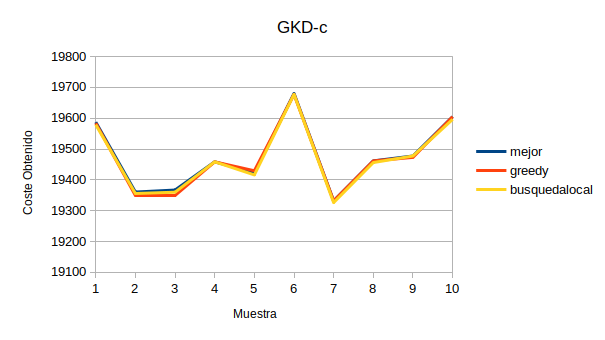
\includegraphics[scale=0.55]{img/gkdc.png}
	\end{figure}
	
	
	
	
	\item \texttt{MDG-a}: Conjunto de datos correspondiente al grupo de distancias enteras y tamaño de $n=2000$ y $m=200$. En todas las muestras los costes obtenidos en el algoritmo de \textit{Búsqueda Local} están por encima de los de \textit{Greedy}, a excepción del archivo \textit{MDG-a\_33}
	
	No hay convergencia en el algoritmo de \textit{BusquedaLocal}, de hecho, éste termina tras realizar 100.000 evaluaciones en la función objetivo. Para explorar el entorno completo se necesitarían $m \cdot (n-m)$ evaluaciones, es decir casi 4 veces más. Sin embargo, el tiempo se hubiera multiplicado por 4 y , por tanto, la calidad del algoritmo sería peor.
	
	
	
	\begin{figure}[H]
		\centering
		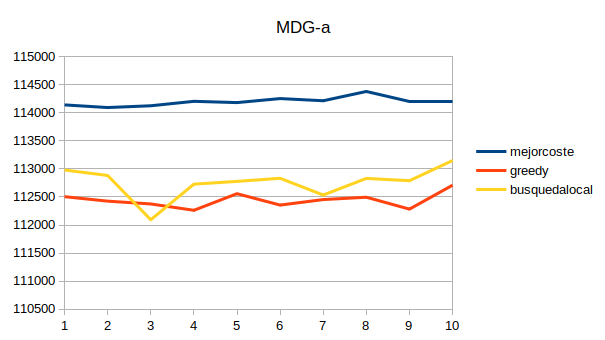
\includegraphics[scale=0.55]{img/mdga.png}
	\end{figure}
	
	
	
	\item \texttt{MDG-b}: Conjunto de datos correspondiente al grupo de distancias reales y tamaño $n=500$ y $m=50$. Al igual que en el caso anterior, el algoritmo de \textit{Búsqueda Local} mejora los costes del algoritmo \textit{greedy}. En este caso, en los archivos centrales del diagrama anterior, la \textit{Búsqueda Local} no mejora los resultados del \textit{greedy}, de hecho, son prácticamente iguales. Esto se debe a la existencia de óptimos locales en nuestro entorno, no permitiendo a nuestro algoritmo de BL salir de éste.
	
	
	\begin{figure}[H]
		\centering
		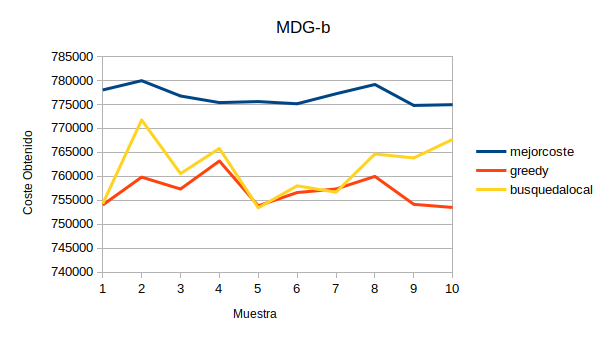
\includegraphics[scale=0.6]{img/mdgb.png}
	\end{figure}
	
\end{itemize}










\subsection{Desviación}
Por último, reflejados en el siguiente gráfico, mostramos en las lineas azules la desviación de la ejecución de cada una de las muestras del algoritmo \textit{Greedy} y, en las líneas naranjas, lo obtenido en la ejecución del algoritmo \textit{Búsqueda Local} que, como bien vemos, se encuentra por debajo (menos en la Muestra 23). 



\begin{figure}[H]
	\centering
	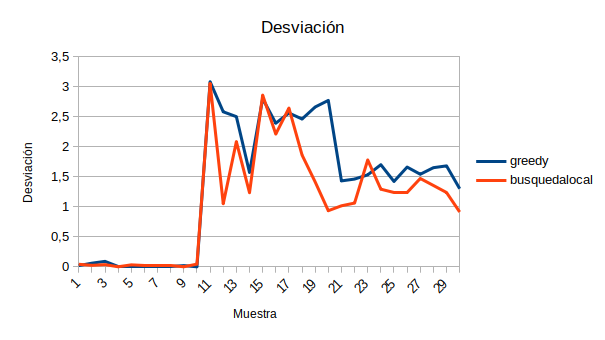
\includegraphics[scale=0.6]{img/desv.png}

\end{figure}

Por otro lado, el área que deja el contorno de la línea naranja es menor que la de la línea azul, pero esto dependerá mucho de la existencia de óptimos locales, que depende a su vez de la solución inicial obtenida. En resumen, podemos considerar que la calidad del algoritmo \textit{Búsqueda Local} es mejor porque en media obtiene soluciones más cercanas al mejor valor conocido.









\newpage





\begin{thebibliography}{X} 
	
-\href{https://sci2s.ugr.es/sites/default/files/files/Teaching/GraduatesCourses/Metaheuristicas/Sem01-Problemas-MHs-2019-20.pdf}{Seminario 1}\\
	
	-\href{https://sci2s.ugr.es/sites/default/files/files/Teaching/GraduatesCourses/Metaheuristicas/Sem02-Problemas-BusquedaLocal-MHs-19-20.pdf}{Seminario 2}\\
	
	-\href{https://sci2s.ugr.es/sites/default/files/files/Teaching/GraduatesCourses/Metaheuristicas/Guion\%20P1a\%20LocalGreedy\%20MDP\%20MHs\%202019-20.pdf}{Guión de prácticas}


\end{thebibliography}


\end{document}

